\section{Python-based Utilities}
\label{sec:pythonutils}
Like many ACRO packages, PEBBL provides some untility programs written in
Python.  These utilities are strictly serial, and reside in the
directories
\begin{codeblock}
~~~~~\=acro-pebbl/packages/pebbl/python/scripts \\
\textrm{and} \>acro-pebbl/python/bin
\end{codeblock}


\subsection{The \texttt{dumpSplit} utility}
\label{sec:dumpsplit}
The \texttt{dumpSplit} utility is helpful for separating logs produced
by setting the \texttt{debug} command-line parameter.  For parallel
runs, PEBBL prefixes each line of output with the MPI process number
enclosed in square brackets.  For example, output lines from processor
0 start with \texttt{[0]}, output lines from processor 1 start with
\texttt{[1]}, and so forth.  These lines typically appear intermixed
in the output.  The \texttt{dumpSplit} utility is meant to assist in
forming a clearer picture of what is happening on each individual
processor.  Its usage is through a command line of the form
\begin{codeblock}
\textit{path}/dumpSplit \textit{logFile}
\end{codeblock}
Here, \texttt{\textit{path}} is the location of the utility (such as
\texttt{acro-pebbl/python/bin} above) and \texttt{\textit{logFile}} is
the pathname of the file containing the PEBBL debug output.  For each
processor $p$ that \texttt{dumpSplit} detects in
\texttt{\textit{logFile}}, it writes a file of the form
\texttt{\textit{logFile}.$p$} containing just the output flagged as
coming from processor $p$.  For example if \texttt{dumpSplit} were to
be run on a file called \texttt{dump.log} containing debug log output
from three processors, its output would be the files
\texttt{dump.log.0}, \texttt{dump.log.1}, and \texttt{dump.log.2}.


\subsection{The \texttt{pebblLoadGraph} utility}
\label{sec:pebblLoadGraph}
The \texttt{pebblLoadGraph} allows you to visualize parallel
performance-tracking data produced by invoking the
\texttt{loadLogSeconds} parameter described in
Section~\ref{sec:debugparams}.  To use this utility, your Python
installation must contain the \texttt{matplotlib} package available at
\url{http://matplotlib.org}.  When PEBBL is run with
\texttt{loadLogSeconds} set to a positive value, performance data are
placed in a file called \texttt{\textit{problemName}.loadLog} in the
current directory, where \texttt{\textit{problemName}} is the name of
the current problem instance, typically derived from the problem
instance filename.  The \texttt{pebblLoadGraph} utility processes such
files to produce either screen or PDF-file graphics.  You invoke this
utility by a command of the form
\begin{codeblock}
\textit{path}/pebblLoadGraph \textrm{[}\textit{options}\textrm{]} 
\textit{file}
\end{codeblock}
where \texttt{\textit{file}} denotes the load-log file produced by the
PEBBL runs.  By default, graphical output is placed in a file whose
name is derived from \texttt{\textit{file}} but ends in \texttt{.pdf}.
The options available in the optional clauses
\texttt{\textit{options}} are extensive and may be viewed in their
entirety by the command
\begin{codeblock}
\textit{path}/pebblLoadGraph --help
\end{codeblock}
The most common options are
\begin{description}
\item[\texttt{--noworkers}] Do not graph subproblem loads at worker
  processors.  The opposite of this option, \texttt{--workers}, is the
  default.
\item[\texttt{--nohubs}] Do not graph subproblem loads at hub
  processors.  The opposite of this option, \texttt{--hubs}, is the
  default.
\item[\texttt{--proc=}$p$]  Only graph loads for processor $p$.  The
  argument $p$ may also take the value \texttt{hubs}, \texttt{workers}
  or \texttt{all}, which is the default.  This parameter may be
  specified multiple times: for example, \texttt{--proc=0 --proc=2}
  will show only information for processors 0 and 2.
\item[\texttt{--bounds=}$p$] Show the known solution bounds (lower
  bound for a minimization problem, upper bound for a maximization
  problem) known at processor $p$.  The $p$ argument is interpreted
  the same way as for the \texttt{--proc} option.
\item[\texttt{--incumbent=}$p$] Show the incumbent values known at
  processor $p$.  The $p$ argument is interpreted the same way as for
  the \texttt{--proc} option.
\item[\texttt{--show}] Show the graphical output on-screen in addition
  to producing the default PDF file.  Requires an active X display
  connection.
\item[\texttt{--startseconds=}$s_1$]  Only show information after
  $s_1$ seconds of PEBBL runtime.
\item[\texttt{--endseconds=}$s_2$]  Only show information before
  $s_2$ seconds of PEBBL runtime elapsed.
\end{description}
Note that separate loads may be displayed for a single processor if it
is both a worker and a hub --- one display indicates subproblems under
control of the worker process and the other indicates subproblems
under control of the hub process.

Figure~\ref{fig:loadGraph} shows the result of running
\texttt{pebblLoadGraph} with its default settings on a logfile
produced by running PEBBL on a difficult knapsack problem using 8 MPI
processors, two of which were designaged as combined worker-hubs, and
the rest as workers.

\begin{figure}[t]
\begin{center}
\vspace{-0.3in}
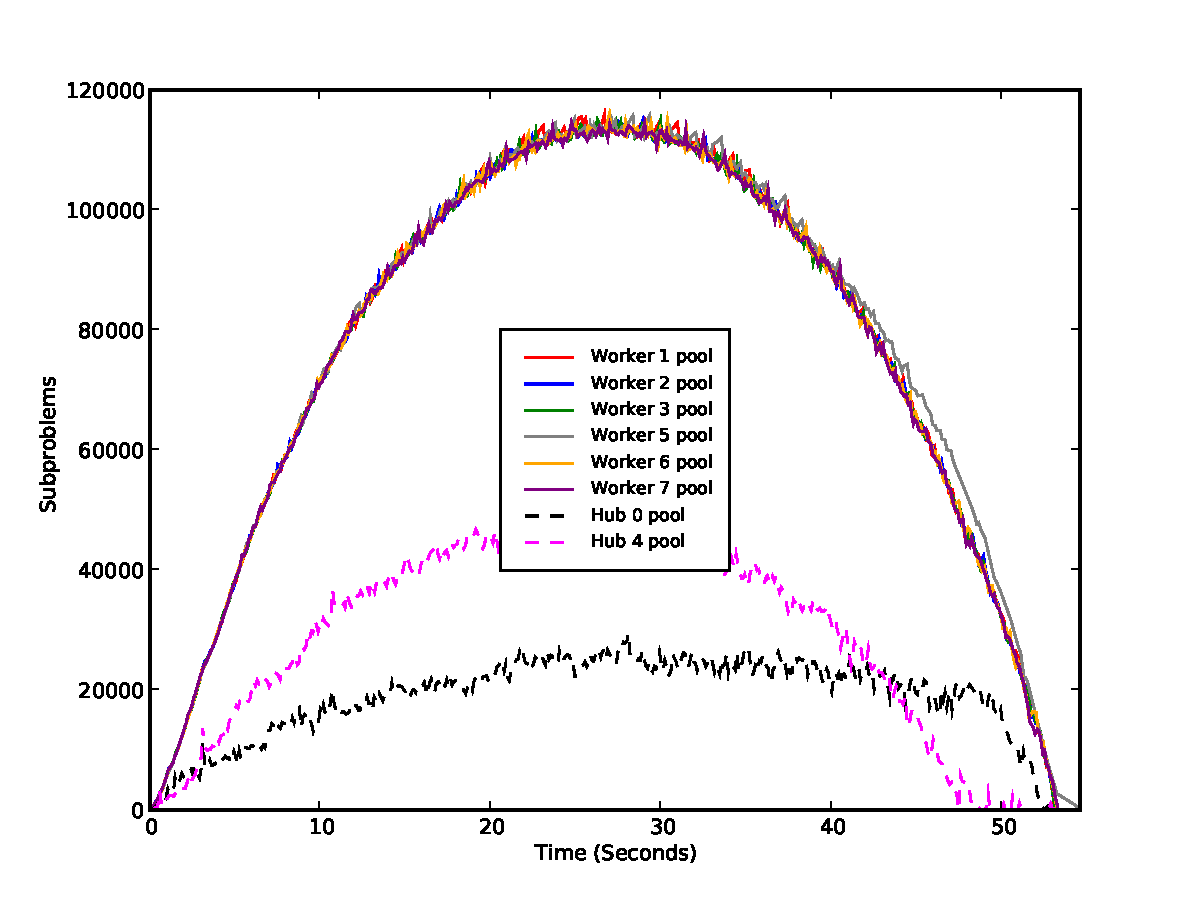
\includegraphics[width=0.95\textwidth]{sample-load-graph}
\vspace{-0.45in}
\end{center}
\caption{Sample graphical output from \texttt{pebblLoadGraph}}.
\label{fig:loadGraph}
\end{figure}
